\section{Evaluation}
\label{sec:experiment}

We perform human evaluation on a multi-axis benchmark for TTT-MLP and five baselines, all with linear complexity: local attention, TTT-Linear, Mamba 2, Gated DeltaNet, and sliding window attention layers.

\subsection{Baselines}
Except for local attention, all baselines are added to the same pre-trained CogVideo-X 5B using the approach in Subection~\ref{subsec:arch}; 
their modified architectures all have 7.2B parameters.
All baselines use the same fine-tuning recipe in Subsection~\ref{subsec:dataset}
and Appendix \ref{sec:appendix:implementation}.
Next we discuss the baselines in detail.
\vspace{0.2em}
\begin{itemize}[itemsep=0.2em]
\item\textbf{Local attention}: No modification to the original architecture, which performs self-attention on each 3-second segment independently.
\item\textbf{TTT-Linear}~\cite{sun2024ttt}: A TTT layer that instantiates $f(x) = x + \texttt{LN}(f_{\,\texttt{Linear}}(x))$, where $f_{\,\texttt{Linear}}$ is a linear model. 
\item\textbf{Mamba 2}~\cite{dao2024mamba2}: A modern RNN layer with a matrix hidden state, which is \(\approx4\times\) larger than the hidden state in TTT-Linear but \(\approx2\times\) smaller than that in TTT-MLP.
\item\textbf{Gated DeltaNet}~\cite{yang2025gateddeltanetworksimproving}: An extension of DeltaNet~\cite{yang2024parallelizing} and Mamba~2 with an improved update rule.
\item\textbf{Sliding-window attention}~\cite{beltagy2020longformerlongdocumenttransformer}: Self-attention with a fixed window of $8192$ tokens (about 1.5 seconds of video). 
% Since CogVideo-X has 42 attention layers, their receptive field covers the entire one-minute context length.
\end{itemize}

\subsection{Evaluation Axes and Protocol}
\label{subsec:quan_eval}
From the six evaluation axes in MovieGen~\cite{meta2024moviegen}, we adopt the four relevant to our domain for human evaluation.\footnote{
Out of the six axes in MovieGen, we omit ``realness" which does not apply to cartoons.
We also omit ``motion completeness" which ``measures whether the output video contains enough motion", because all videos in our domain have highly dynamic motion.
We adapt ``frame consistency" to ``temporal consistency" to also include consistency across scenes.}

\begin{landscape}
\begin{figure}
    \centering
    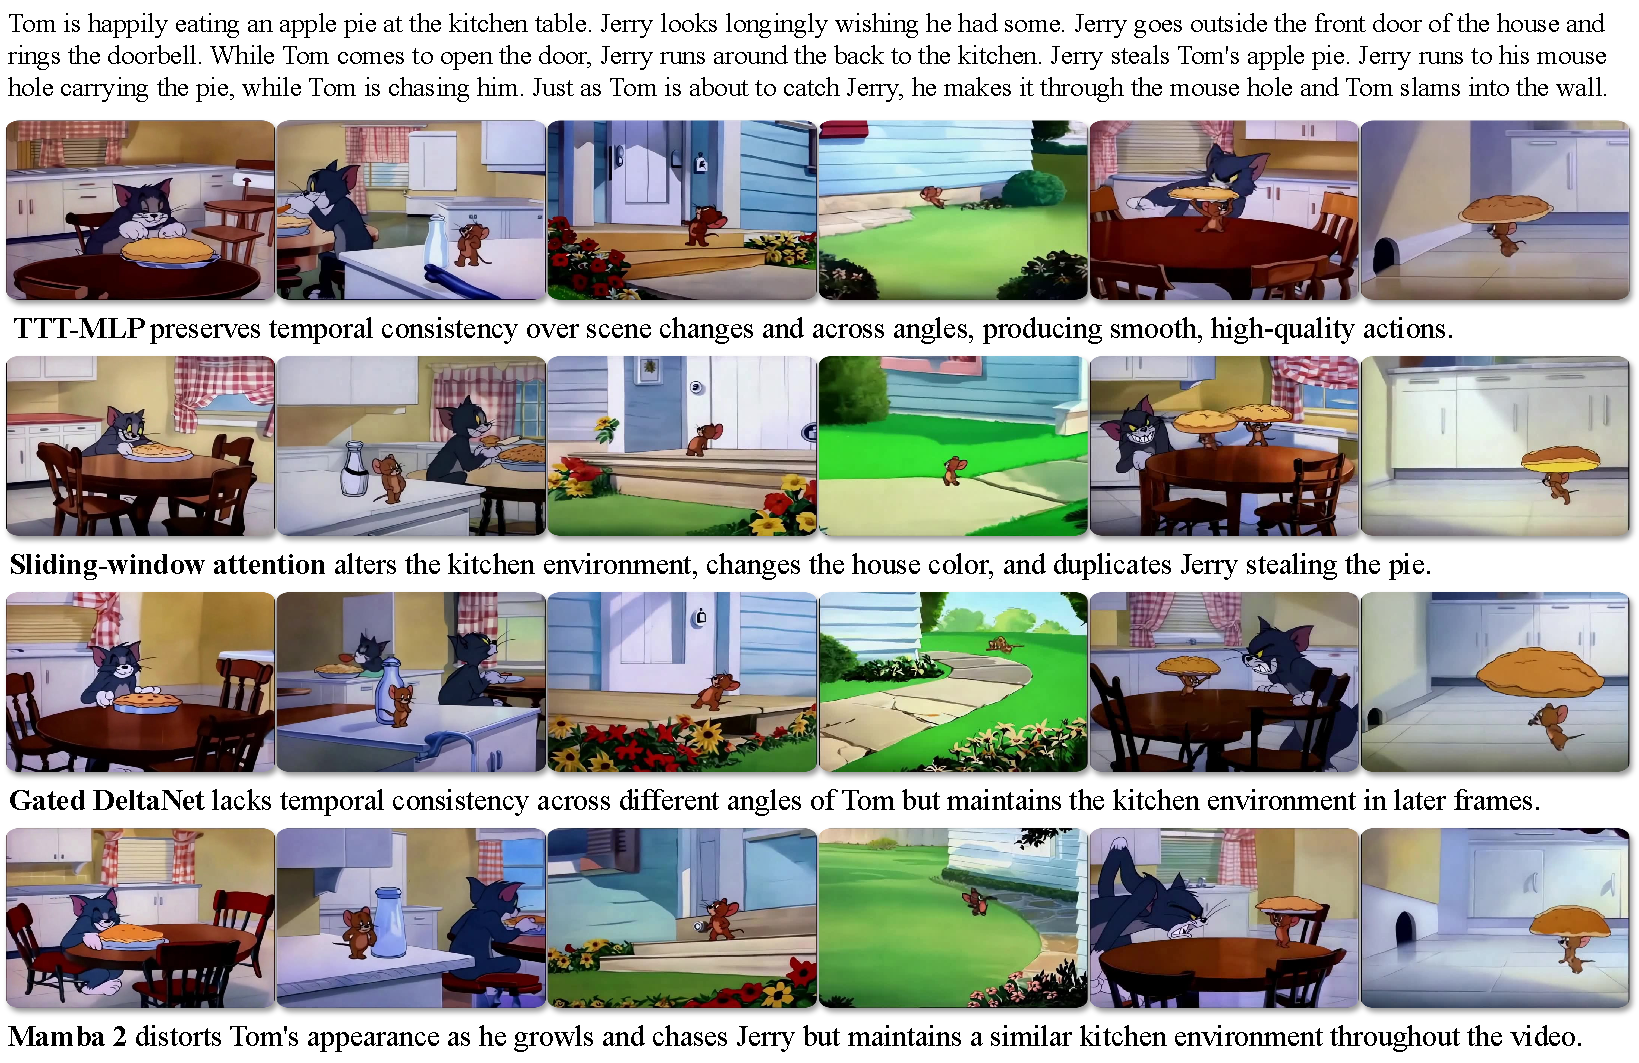
\includegraphics[width=1.28\textwidth]{figs/qualitative.pdf}
    \caption{Video frames comparing TTT-MLP against Gated DeltaNet and sliding-window attention, the leading baselines in our human evaluation. 
    TTT-MLP demonstrates better scene consistency by preserving details across transitions and better motion naturalness by accurately depicting complex actions.}
    \label{fig:qualitative}
\end{figure}
\end{landscape}

\twocolumn[{
\centering
\setlength{\tabcolsep}{6pt}
\renewcommand{\arraystretch}{1.3}
\begin{tabular}{lcccc|c}
    \toprule
     & Text following & Motion naturalness & Aesthetics & Temporal consistency & Average \\
    \midrule
    {Mamba 2} & 985 & 976 & 963 & 988 & 978  \\
    {Gated DeltaNet} & 983 & 984 & 993 & 1004 & 991 \\
    {Sliding window} & \textbf{1016} & 1000 & 1006 & 975 & 999 \\
    {TTT-MLP} & 1014 & \textbf{1039} & \textbf{1037} & \textbf{1042} & \textbf{1033} \\
    \bottomrule
    \end{tabular}
    \captionof{table}{Human evaluation results for one-minute videos. TTT-MLP improves over the second best method by 34 Elo points on average. 
    Axes with the most improvements are scene consistency (+38) and motion smoothness (+39). For context, GPT-4 scores 46 Elo points over GPT-3.5 Turbo, and GPT-4o scores 29 over GPT-4 Turbo in Chatbot Arena~\cite{chiang2024chatbot}.}
    \label{tab:multiaxis_evaluation}

    \begin{minipage}[c]{0.66\textwidth}
    \vspace{2ex}
        \includegraphics[width=\linewidth]{figs/latency.pdf}
    \end{minipage}\hfill
    \begin{minipage}[c]{0.33\textwidth}
    \vspace{2ex}
        \captionof{figure}{
        For 63-second videos, inference with full attention (over 300k tokens) would have taken $11\times$ longer than local attention, and training $12\times$ longer, as discussed in Section~\ref{sec:intro}.
        TTT-MLP takes $2.5\times$ and $3.8\times$ respectively -- significantly more efficient than full attention, but still less efficient than, for example, Gated DeltaNet, which takes $1.8\times$ longer than local attention in both inference and training.
        }
        \label{fig:your_label}
    \end{minipage}
    \vspace{1.0em}
}]

\begin{itemize}[itemsep=0.2em]
\item \textbf{Text following}: ``aligment with the provided prompt."
\item \textbf{Motion naturalness}: ``natural limb
movements, facial expressions, and adherence to physical laws.
Motion that appears unnatural or uncanny will be penalized."
\item \textbf{Aesthetics}: ``interesting and compelling content, lighting, color, and camera effects."
\item \textbf{Temporal consistency}: both inside and across scenes.
\end{itemize}
The quoted descriptions are from MovieGen~\cite{meta2024moviegen}.


Our evaluation is based on pairwise preferences in blind comparisons, because directly rating long videos or ranking many of them at once is challenging.
Specifically, an evaluator is given a random axis from the four above and a random pair of videos sharing the same plot, then asked to indicate the better video for that axis.
To collect the pool of videos, we first sample 100 plots using Claude 3.7 Sonnet (in Format $1\rightarrow2\rightarrow3$ as discussed in Subsection~\ref{subsec:pipeline}), then generate one video per method per plot.
The methods generating the videos are always unknown to the evaluators.

Our evaluators were recruited on \texttt{prolific.com} with the filters: living in the U.S., English as a first language, aged 18 to 35 years, with at least 100 previous submissions and an approval rate of at least 98\%.
The demographics of our evaluators, disclosed on the website, are as follows.
\vspace{0.2em}
\begin{itemize}[itemsep=0.2em]
\item \textbf{Gender}: 50.78\% male, 47.66\% female, 1.56\% other.
\item \textbf{Ethnicity}: 57.03\% White, 23.44\% Black, 10.94\% Mixed, 5.47\% Asian, and 3.12\% other. 
\end{itemize}
Based on this information, we believe that our evaluators constitute a representative sample of the U.S. population.

\begin{figure*}[!t]
    \centering
    \includegraphics[width=\textwidth]{figs/limitations.pdf}
    \vspace{-10pt}
    \caption{Artifacts in videos generated by TTT-MLP. 
    \textbf{Temporal consistency}: Objects sometimes morph at the boundaries of 3-second segments, potentially because the diffusion model samples from different modes across the segments.
    \textbf{Motion naturalness}: Objects sometimes float unnaturally because gravitational effects are not properly modeled.
    \textbf{Aesthetics}: Lighting changes do not consistently align with actions unless explicitly prompted. 
    Complex camera movements, such as parallax, are sometimes depicted inaccurately.
    }
    \label{fig:limitations}
\end{figure*}

\subsection{Results}
\label{subsec:results}

We aggregate the pairwise preferences using the Elo system in LMSys Chatbot Arena~\cite{chiang2024chatbot}.
The Elo scores are shown in Table~\ref{tab:multiaxis_evaluation}.

TTT-MLP improves over the second-best method by 34 Elo points on average. 
For context, GPT-4 scores 46 Elo points over GPT-3.5 Turbo (1163 vs. 1117), and GPT-4o scores 29 over GPT-4 Turbo (1285 vs. 1256) in LMSys Chatbot Arena~\cite{chiang2024chatbot}, so our improvement by 34 is practically meaningful.\footnote{
\url{https://lmarena.ai/}, accessed on March 20, 2025. The models considered are
GPT-4o-2024-05-13,
GPT-4-Turbo-2024-04-09,
GPT-4-0613, and
GPT-3.5-Turbo-0613.
}
Figure~\ref{fig:qualitative} compares frames of sample videos generated by TTT-MLP and the baselines.
The videos illustrated in Figure~\ref{fig:qualitative} can be accessed on the project website:
\url{https://test-time-training.github.io/video-dit}

\myparagraph{18-second elimination round.}
Note that local attention and TTT-Linear do not appear in Table~\ref{tab:multiaxis_evaluation}.
To avoid the much higher cost of evaluating longer videos on every method, we first conducted an elimination round using 18-second videos following the same procedure discussed in Subsection~\ref{subsec:quan_eval}.
This round eliminated local attention, which performed worst, and also TTT-Linear, which performed worse than TTT-MLP.
Results of the elimination round are shown in Table~\ref{tab:appendix:multiaxis_evaluation} in the Appendix.

\subsection{Limitations}
\label{subsec:limitations}
\myparagraph{Short context.}
For the 18-second elimination round discussed above, Gated DeltaNet performs the best on average, leading Mamba~2 by 27 Elo points and TTT-MLP by 28 (see Table~\ref{tab:appendix:multiaxis_evaluation} in the Appendix).
For 18-second videos, the context length is roughly 100k tokens.
This evaluation shows the scenario where RNN layers with linear (matrix) hidden states, such as Gated DeltaNet and Mamba~2, are still the most effective.
Moreover, evaluation results for both 18 and 63-second videos indicate that Gated DeltaNet improves meaningfully on Mamba~2.

\myparagraph{Wall-clock time.}
Even after applying our improvements in Subsection~\ref{subsec:parallel} and \ref{subsec:gpu}, the efficiency of TTT-MLP is still worse than Gated DeltaNet and Mamba~2.
This limitation is highlighted in Figure~\ref{fig:your_label}, where inference and training with TTT-MLP are $1.4\times$ and $2.1\times$ slower than with Gated DeltaNet, for example.
Section~\ref{sec:conclusion} discusses two potential improvements of our TTT-MLP kernel for better efficiency.
Note that training efficiency is not a significant concern in our application because the RNN layers are integrated after pre-training, which constitutes most of the overall training budget.
Training efficiency of the RNN layers is only relevant during fine-tuning, which is a small part of the budget to begin with.
In contrast, inference efficiency is much more meaningful.

\myparagraph{Video artifacts.}
The generated 63-second videos demonstrate clear potential as a proof of concept, but still contain notable artifacts, especially in motion naturalness and aesthetics. Figure~\ref{fig:limitations} illustrates examples of artifacts corresponding to three of our evaluation axes.
We observe that videos with these kinds of artifacts are not particular to TTT-MLP, but common among all methods.
The artifacts might have been a consequence of the limited capability of the pre-trained CogVideo-X 5B model.
For example,
videos (\href{https://github.com/THUDM/CogVideo}{link}) generated by the original CogVideo-X also seem to have limited motion naturalness and aesthetics.
